\documentclass[11pt]{article}

% common LaTeX macros
%
% Last modified: 03-02-2007
%

\usepackage{times}
%-------------------------
% the following magic makes the tt font in math mode be the same as the
% normal tt font (i.e., Courier)
%
\SetMathAlphabet{\mathtt}{normal}{OT1}{pcr}{n}{n}
\SetMathAlphabet{\mathtt}{bold}{OT1}{pcr}{bx}{n}
%-------------------------

\usepackage{amsmath}
\usepackage{amssymb} % for \pitchfork

\newcommand{\NOTE}[1]{%
  \par\leavevmode\noindent\textbf{[[ #1 ]]}\par\leavevmode\noindent}
\newcommand{\CUT}[1]{}
\newcommand{\SIDENOTE}[1]{%
  \marginpar{\tiny\raggedright{#1}}}

\newcommand{\appref}[1]{Appendix~\ref{#1}}
\newcommand{\chapref}[1]{Chapter~\ref{#1}}
\newcommand{\secref}[1]{Section~\ref{#1}}
\newcommand{\tblref}[1]{Table~\ref{#1}}
\newcommand{\figref}[1]{Figure~\ref{#1}}
\newcommand{\listingref}[1]{Listing~\ref{#1}}
\newcommand{\pref}[1]{{page~\pageref{#1}}}
\newcommand{\defref}[1]{Definition~\ref{#1}}
\newcommand{\ruleref}[1]{Rule~\ref{#1}}

\newcommand{\eg}{{\em e.g.}}
\newcommand{\cf}{{\em cf.}}
\newcommand{\ie}{{\em i.e.}}
\newcommand{\etc}{{\em etc.\/}}
\newcommand{\naive}{na\"{\i}ve}
\newcommand{\ala}{{\em \`{a} la\/}}
\newcommand{\etal}{{\em et al.\/}}
\newcommand{\role}{r\^{o}le}
\newcommand{\vs}{{\em vs.}}
\newcommand{\forte}{{fort\'{e}\/}}

%
% language names
\newcommand{\Cplusplus}{\mbox{C\hspace{-.05em}\raisebox{.4ex}{\tiny\bf ++}}}
\newcommand{\Cmm}{\mbox{C\hspace{-.05em}\raisebox{.4ex}{\small\textbf{{-}{-}}}}}
\newcommand{\csharp}{\textsc{C\#}}
\newcommand{\C}{\textsc{C}}
\newcommand{\Ckit}{\textsc{Ckit}}
\newcommand{\java}{\textsc{Java}}
\newcommand{\loom}{\textsc{Loom}}
\newcommand{\moby}{\textsc{Moby}}
\newcommand{\minimoby}{\textsc{MiniMoby}}
\newcommand{\micromoby}{\textsc{microMoby}}
\newcommand{\MOC}{\textsc{MOC}}
\newcommand{\ml}{\textsc{ML}}
\newcommand{\sml}{\textsc{SML}}
\newcommand{\smlnj}{\textsc{SML/NJ}}
\newcommand{\mlj}{\textsc{MLj}}
\newcommand{\cml}{\textsc{CML}}
\newcommand{\pml}{\textsc{PML}}
\newcommand{\ocaml}{\textsc{OCaml}}
\newcommand{\mlkk}{\textsc{ML2000}}
\newcommand{\haskell}{\textsc{Haskell}}
\newcommand{\mltwok}{\textsc{ML2000}}
\newcommand{\scala}{\textsc{Scala}}
\newcommand{\perl}{\textsc{Perl}}
\newcommand{\scheme}{\textsc{Scheme}}
\newcommand{\unix}{\textsc{Unix}}
\newcommand{\smalltalk}{\textsc{Smalltalk}}
\newcommand{\self}{\textsc{Self}}

%
% font commands
\providecommand{\bftt}[1]{{\ttfamily\bfseries{}#1}}
\providecommand{\ittt}[1]{{\ttfamily\itshape{}#1}}
\providecommand{\kw}[1]{\bftt{#1}}
\providecommand{\nt}[1]{{\rmfamily\itshape{#1}}}
\providecommand{\term}[1]{{\sffamily{#1}}}
%
% math-mode versions
\providecommand{\mkw}[1]{\ensuremath{\text{\kw{#1}}}}
\providecommand{\mnt}[1]{\ensuremath{\text{\nt{#1}}}}
\providecommand{\mterm}[1]{\ensuremath{\text{\term{#1}}}}

% braces (in math mode)
\newcommand{\LCB}{\mkw{\{}}
\newcommand{\RCB}{\mkw{\}}}

% underscore
\newcommand{\US}{\char`\_}

%%%%%
% Some common math notation
%

% double brackets
\newcommand{\LDB}{\ensuremath{[\mskip -3mu [}}
\newcommand{\RDB}{\ensuremath{]\mskip -3mu ]}}

\newcommand{\dom}{\ensuremath{\mathrm{dom}}}
\newcommand{\rng}{\ensuremath{\mathrm{rng}}}

% sets
\newcommand{\SET}[1]{\ensuremath{\{#1\}}}
\newcommand{\Fin}{\textrm{Fin}}     % finite power set
\newcommand{\DISJOINT}[2]{\ensuremath{#1 \pitchfork #2}}
\newcommand{\finsubset}{\mathrel{\stackrel{\textrm{fin}}{\subset}}}


% finite maps
\newcommand{\finmap}{\mathrel{\stackrel{\textrm{fin}}{\rightarrow}}}
\newcommand{\MAP}[2]{\SET{#1 \mapsto #2}}
\newcommand{\EXTEND}[2]{\ensuremath{#1{\pm}#2}}
\newcommand{\EXTENDone}[3]{\EXTEND{#1}{\MAP{#2}{#3}}}
\newcommand{\SUBST}[3]{\ensuremath{#1[#2\mapsto{}#3]}}
\newcommand{\SUBSTTWO}[5]{\ensuremath{#1[#2\mapsto{}#3,#4\mapsto{}#5]}}


% timestamp
\newcount\timeHH
\newcount\timeMM
\timeHH=\time
\divide\timeHH by 60
\timeMM=\time
\count255=\timeHH
\multiply\count255 by -60 \advance\timeMM by \count255
\newcommand{\timestamp}{%
  \today{} ---
  \ifnum\timeHH<10 0\fi\number\timeHH\,:\,\ifnum\timeMM<10 0\fi\number\timeMM}


\usepackage{graphicx}

\title{VProc protocol}
\author{The Manticore Group}
\date{Draft of \today}

\begin{document}
\maketitle

\section{Overview}

\begin{figure}[tp]
  \begin{center}
    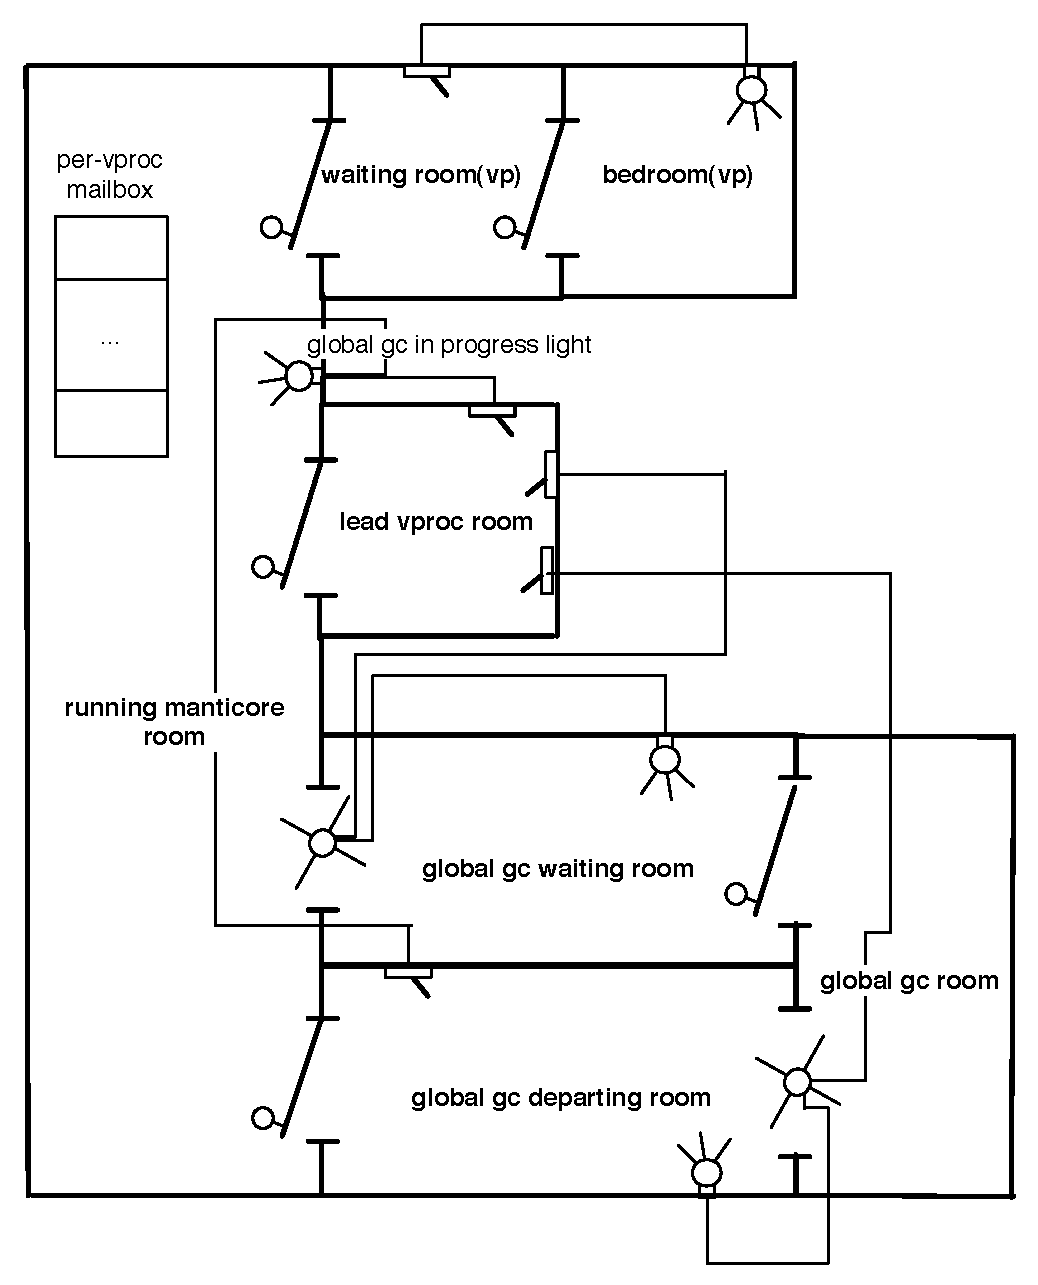
\includegraphics[scale=0.7]{pictures/vproc-protocol}
  \end{center}%
  \caption{Layout of the VProc protocol.}
  \label{fig:vproc-protocol}
\end{figure}%

\section{Messaging}

\paragraph{\texttt{Send(vp, msg)}}

\begin{description}
\item [\textit{Precondition:}] \textit{It is the case that} \texttt{vp} $\neq$ \texttt{host\_vproc} \textit{(a vproc cannot send a message to itself)}
\end{description}

\begin{enumerate}
  \item Walk to \texttt{vp}'s desk and open the mailbox.
    \begin{enumerate}
      \item If there is a \texttt{SLEEPING} message, place \texttt{msg} in the mailbox and go to step 2.
      \item Otherwise, place \texttt{msg} in the mailbox and exit the subroutine.
    \end{enumerate}
  \item Walk into \texttt{vp}'s \textbf{waiting room}.
    \begin{enumerate}
      \item If the waiting-room switch is off, then do the following. \textit{(\textbf{Invariant:}} \texttt{vp} \textit{is on its way to the waiting room.)}
        \begin{enumerate}
          \item Flip the waiting-room switch on.
          \item Return to the local desk.
          \item Exit the subroutine.
        \end{enumerate}
      \item If the waiting-room switch is on, then go to step 3. \textit{(\textbf{Invariant:}} \texttt{vp} \textit{is in its bedroom.)}
    \end{enumerate}
  \item Flip the bedroom switch on.
  \item Return to the local desk.
\end{enumerate}

\begin{description}
\item [\textit{Postcondition:}] \textit{At some point in the future,} \texttt{vp} \textit{will sit at its desk and open} \texttt{msg}.
\end{description}

\paragraph{\texttt{CheckMailbox()}}

\begin{enumerate}
  \item Open the local mailbox.
  \item Retrieve all messages, leaving the mailbox empty.
  \item Handle each message \texttt{msg}.
\end{enumerate}

\section{Sleeping}

\paragraph{\texttt{Sleep()}}

\begin{enumerate}
  \item Walk to the desk and open the mailbox.
    \begin{itemize}
      \item If empty, place a \texttt{SLEEPING} message in the mailbox.
      \item If nonempty, exit the subroutine.
    \end{itemize}
  \item Walk into the \textbf{waiting room}.
    \begin{itemize}
      \item If the waiting-room switch is on, then go to step 7. \textit{(\textbf{Invariant:}} \textit{Another vproc has delivered mail and has just walked out of the \textbf{waiting room}.)}
      \item If the waiting-room switch is off, then go to step 3. \textit{(\textbf{Invariant:}} \textit{It is the case that, in the time between the current step and step 1, no other vproc has entered the \textbf{waiting room}.)}
    \end{itemize}
  \item Flip the bedroom switch off.
  \item Walk into \textbf{bedroom}.
  \item Wait for the light to turn on.
  \item Walk into \textbf{waiting room}.
  \item Flip the waiting-room switch off.
  \item Return to the desk.
\end{enumerate}

\paragraph{\texttt{Wake(vp)}}

\begin{enumerate}
  \item Construct a blank message \texttt{msg}.
  \item Apply \texttt{Send(vp, msg)} and, once complete, exit the subroutine.
\end{enumerate}

\section{Global GC}

\paragraph{\texttt{GlobalLimit()}}

\begin{enumerate}
  \item Walk into \textbf{leader vproc room}.
    \begin{itemize}
      \item If switch is off, then we assign this vproc as the lead.
        \begin{enumerate}
          \item Flip the global-gc switch on.
          \item Reset turnstyles.
          \item Leave the \textbf{leader vproc room}.
          \item Go to \texttt{LeaderVProc()}.
        \end{enumerate}
      \item If switch is on, then go to step 2.
    \end{itemize}
  \item Walk into \textbf{global gc waiting room}.
  \item Wait for light to turn on.
  \item Enter \textbf{global gc room}.
  \item When finished with global collection, walk to \textbf{global gc departing room}.
  \item Wait for light to turn on.
  \item Return to the desk.
\end{enumerate}

\paragraph{\texttt{LeaderVProc()}}

\begin{enumerate}
  \item For each vproc \texttt{vp}, apply \texttt{Wake(vp)}.
  \item Walk into \textbf{global gc waiting room}.
  \item Wait for light to turn on.
  \item Walk into \textbf{global gc room}.
  \item When finished with global collection, walk to \textbf{global gc departing room}.
  \item Flip the switch off.
  \item Wait for light to turn on.
  \item Return to the desk.
\end{enumerate}

\end{document}  
